\documentclass[11pt,a4paper]{article}
\usepackage[margin=2.4cm]{geometry}
\usepackage[T1]{fontenc}
\usepackage{lmodern}
\usepackage{amsmath,amssymb,amsthm,mathtools,bm}
\usepackage{booktabs}
\usepackage{tikz}
\usetikzlibrary{positioning,fit,arrows.meta,backgrounds,shapes.geometric,calc}
\usepackage[numbers,sort&compress]{natbib}
\usepackage{xcolor}
\usepackage[colorlinks=true,linkcolor=blue!50!black,citecolor=blue!50!black,urlcolor=blue!50!black]{hyperref}

% ---------------------------------------------------------------------
% Vocabulary note. This version uses only the probability vocabulary of
% Bertsekas & Tsitsiklis, "Introduction to Probability" (MIT 6.041 notes,
% Fall 2000), cited as [BT]. Every probabilistic notion is either taken
% from [BT] or defined in place from [BT] notions. Poker and game-theory
% terms (equilibrium, best response, exploitability) are domain terms and
% are kept.
% ---------------------------------------------------------------------

\setlength{\emergencystretch}{2em}

\newtheorem{proposition}{Proposition}
\newtheorem{definition}{Definition}
\newtheorem{remark}{Remark}

\newcommand{\C}{C}            % opponent hole cards
\newcommand{\Sb}{S}           % strength bucket
\newcommand{\Z}{Z}            % style
\newcommand{\A}{A}            % action
\newcommand{\X}{X}            % public context
\newcommand{\B}{B}            % board
\newcommand{\R}{R}            % reveal variable
\newcommand{\E}{\mathbf{E}}
\newcommand{\1}{\mathbf{1}}
\newcommand{\BT}[1]{\cite[§#1]{bertsekas2000}}
\newcommand{\todo}[1]{\textcolor{red!70!black}{[TODO: #1]}}

\title{Reading the Whole Hand:\\
A Two-Timescale Probabilistic Model of One Opponent\\
in Heads-Up Limit Hold'em, with Hidden Cards Handled Correctly}
\author{Draft --- \today}
\date{}

\begin{document}
\maketitle

\begin{abstract}
Since 1999, poker programs have used probabilistic models to infer an opponent's
unseen cards from the betting. These models share three recurring defects.
They learn only from hands that reach showdown. They treat each betting round,
or even each single action, separately. And they assume that the opponent's
style never changes. We propose a \emph{two-timescale probabilistic model}.
Within a hand, Bayes' rule is applied exactly, action by action, to the
conditional PMF of the opponent's $1326$ possible hole-card pairs, using
hand-strength features that are recomputed on every street. Across hands, an
unobserved \emph{style} variable evolves as a Markov chain that rarely changes
state, which captures shifts such as tilt. Whether the cards are revealed is
completely determined by the observed betting. We show that, for this reason,
the hidden cards of folded hands can be summed out by the total probability
theorem without distorting what is learned. Parameters fitted this way converge
in probability to the true ones. By contrast, the showdown-only frequency
estimator used in earlier work converges to a provably wrong value. We confirm
this error on $120{,}000$ Annual Computer Poker Competition (ACPC) hands, in
which all hole cards are revealed. On top of the conditional PMF we define:
(i)~\emph{decision certificates}, the conditional probability, given everything
observed, that a recommended action is the best one, exact on the river;
(ii)~an exact additive split of the change in the odds of an event across the
individual actions; and (iii)~\emph{pattern statistics}: bluff and slow-play
indices, model comparisons that test whether the opponent's play depends on a
given variable, and detection of style changes during play. This draft fixes
the model, the computations for learning and inference, and the evaluation
protocol.
\end{abstract}

%=====================================================================
\section{Introduction}
%=====================================================================

Terry and Mihok~\cite{terry2005} built a seven-variable probabilistic model that
infers an opponent's Limit Hold'em holding from a \emph{single} action, fitted to
$476{,}468$ showdown records. They report low accuracy and diagnose the cause
themselves: the model has no memory of the earlier betting, its probabilities
ignore the street, and it has no decision layer. As future work they propose a
model that evolves over time. The Monash Bayesian Poker
Player~\cite{korb1999,nicholson2006} added a full decision layer but learned its
opponent model only from showdowns, and acknowledged that showdown hands are an
unrepresentative selection. Heiberg~\cite{heiberg2013} proposed taking the
expected values of the unrevealed hands into account, together with a
street-to-street chain of conditional PMFs, but reported no results. Southey et
al.~\cite{southey2005} handled folded hands correctly, by summing over the
unseen cards, but assumed an opponent whose behaviour never changes.

Meanwhile, superhuman equilibrium agents~\cite{bowling2015,moravcik2017,brown2018,brown2019,brown2020}
perform the same Bayes'-rule update of the opponent's possible holdings, but
with the equilibrium strategy supplying the conditional probabilities of the
actions. By design they do not model or exploit a particular opponent, and they
give no human-readable reason for a decision.

This project targets the part those systems leave out: a \textbf{well-calibrated,
interpretable, time-aware probabilistic model of one opponent}, together with a
decision layer that can \emph{justify} its recommendations. Contributions:

\begin{enumerate}
  \item A two-timescale model (Section~\ref{sec:model}). Within each hand, the
        conditional PMF of the hole cards is updated exactly, using
        street-dependent strength features. Across hands, a Markov chain models
        the opponent's unobserved style.
  \item A proof that hiding the cards of folded hands does no harm once those
        cards are summed out, and a closed-form expression for the error of the
        showdown-only estimator (Section~\ref{sec:censoring}), confirmed on ACPC
        data (Section~\ref{sec:prelim}).
  \item An iterative expected-count procedure for learning the parameters, which
        are themselves modelled as continuous random variables, and a recursive
        update for use during play (Section~\ref{sec:learning}).
  \item Decision certificates, an exact split of the evidence, and
        ``what-if'' explanations (Section~\ref{sec:decisions}); pattern
        statistics and detection of style changes (Section~\ref{sec:patterns}).
  \item An evaluation protocol with known true answers at three scales: Kuhn
        poker (closed form), Leduc Hold'em (exact exploitability), and ACPC
        heads-up limit Hold'em with the hiding of folded hands simulated
        (Section~\ref{sec:eval}).
\end{enumerate}

All probabilistic tools used are those of~\cite{bertsekas2000}. Appendix~\ref{app:tools}
lists them by section.

%=====================================================================
\section{Setting and notation}
%=====================================================================

We consider heads-up fixed-limit Texas Hold'em (HULHE). We are the
\emph{observer}~$\mathsf{O}$, playing against opponent~$\mathsf{P}$ over a session
of hands $h=1,\dots,H$. Streets are $t\in\{0,1,2,3\}$ (preflop, flop, turn,
river). Each hand is one run of an experiment whose outcome lists all cards and
all actions~\BT{1.2}. The quantities below are random variables, that is,
functions of this outcome~\BT{2.1}. For hand $h$:

\begin{itemize}
  \item $\C_h\in\mathcal{C}$ is the opponent's hole-card pair. There are
        $|\mathcal{C}|=\binom{52}{2}=1326$ such pairs, a count of
        combinations~\BT{1.6}. $o_h$ denotes our hole cards and $\B_{h,t}$ the
        board after street $t$ is dealt ($|\B_{h,0}|=0$, then $3,4,5$ cards).
  \item $\mathcal{C}(o_h,\B_{h,t})\subset\mathcal{C}$ is the set of pairs that
        share no card with the visible cards (card removal).
  \item $\Sb_{h,t}=\phi_t(\C_h,\B_{h,t})\in\{1,\dots,K\}$ is a \emph{strength
        bucket}. It is a function of random variables, hence itself a random
        variable~\BT{2.3}. One example is the rank of the expected value of the
        squared hand strength (E[HS$^2$]) on street~$t$, cut into $K$ bins of
        equal probability~\cite{johanson2013}. Preflop, $\phi_0$ groups the 169
        distinct starting hands.
  \item $\A_{h,t,j}$ is the opponent's $j$-th action on street $t$. The legal
        sets are $\mathcal{L}(x)=\{\mathtt{c},\mathtt{r}\}$ (check, bet) when
        not facing a bet, $\{\mathtt{f},\mathtt{c},\mathtt{r}\}$ (fold, call,
        raise) when facing one, and $\{\mathtt{f},\mathtt{c}\}$ at the four-bet
        cap.
  \item $\X_{h,t,j}=(t,\ \text{facing},\ \text{raises so far},\ \text{position},\
        \text{texture}(\B_{h,t}))$ is the public context of that decision. It is
        a function of the public history and involves no further randomness.
  \item $\R_h\in\{0,1\}$ equals $1$ if $\C_h$ is revealed. In HULHE with forced
        showing (as in ACPC), $\R_h=1$ exactly when no player folds.
  \item $\Z_h\in\{1,\dots,M\}$ is the opponent's unobserved \emph{style} during
        hand $h$, for example \{baseline, loose-aggressive, tight-passive\}.
\end{itemize}

Our own actions are observed. We treat them as given inputs, not as random
variables of the model; they enter only through $\X$. We write $\mathbf{a}_h$
for all opponent actions in hand $h$. $\mathcal{O}_h$ denotes the event that
everything observed in hand $h$ takes its experimental value: $o_h$, the boards,
all actions, and $\C_h$ if $\R_h=1$. $\mathcal{O}_{1:h}$ denotes the
intersection of these events over the session so far.

%=====================================================================
\section{The two-timescale model}\label{sec:model}
%=====================================================================

\begin{figure}[t]
\centering
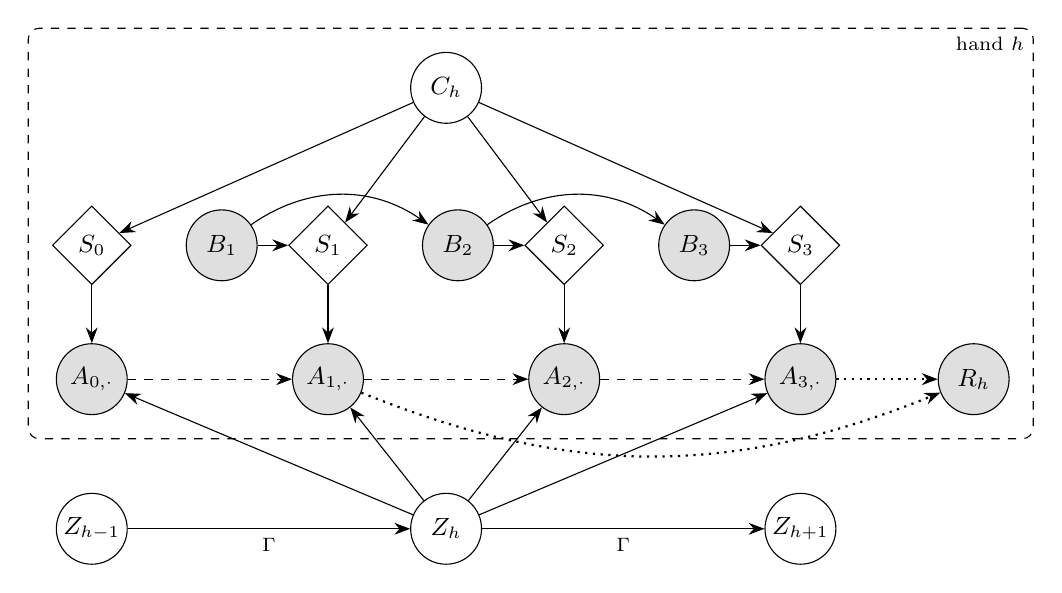
\begin{tikzpicture}[
  >={Stealth[length=2mm]},
  hid/.style={circle,draw,minimum size=9mm,inner sep=0pt,font=\small},
  obs/.style={circle,draw,fill=gray!25,minimum size=9mm,inner sep=0pt,font=\small},
  det/.style={diamond,draw,minimum size=10mm,inner sep=0pt,font=\small}]
  % hand level
  \node[hid] (C) at (4.5,0) {$\C_h$};
  \foreach \t in {0,1,2,3} {
    \node[det] (S\t) at (3*\t,-2) {$\Sb_{\t}$};
    \node[obs] (A\t) at (3*\t,-3.7) {$\A_{\t,\cdot}$};
    \draw[->] (C) -- (S\t);
    \draw[->] (S\t) -- (A\t);
  }
  \foreach \t in {1,2,3} {
    \node[obs] (B\t) at (3*\t-1.35,-2) {$\B_{\t}$};
    \draw[->] (B\t) -- (S\t);
  }
  \draw[->] (B1) to[bend left=35] (B2);
  \draw[->] (B2) to[bend left=35] (B3);
  \foreach \t/\u in {0/1,1/2,2/3} { \draw[->,dashed] (A\t) -- (A\u); }
  \node[obs] (R) at (11.2,-3.7) {$\R_h$};
  \draw[->,dotted,thick] (A3) -- (R);
  \draw[->,dotted,thick] (A1) to[bend right=22] (R);
  % session level
  \node[hid] (Z) at (4.5,-5.6) {$\Z_h$};
  \node[hid] (Zp) at (0,-5.6) {$\Z_{h-1}$};
  \node[hid] (Zn) at (9,-5.6) {$\Z_{h+1}$};
  \draw[->] (Zp) -- node[below,font=\scriptsize]{$\Gamma$} (Z);
  \draw[->] (Z) -- node[below,font=\scriptsize]{$\Gamma$} (Zn);
  \foreach \t in {0,1,2,3} { \draw[->] (Z) -- (A\t); }
  \begin{scope}[on background layer]
    \node[draw,rounded corners,dashed,fit=(C)(S0)(A0)(A3)(B1)(R),inner sep=3mm,
          label={[font=\scriptsize,anchor=north east]north east:hand $h$}] {};
  \end{scope}
\end{tikzpicture}
\caption{Sequential description of the model. An arrow $U\to V$ means that the
model specifies the conditional PMF of $V$ given $U$; reading the arrows in
order gives the multiplication rule~\BT{1.3}. Shaded: observed random
variables. Diamonds: strength features $\Sb_t=\phi_t(\C,\B_t)$, which are
functions of their parents and add no randomness. Within a hand, the single
unobserved pair $\C_h$ affects every street. Dashed arrows carry the public
context $\X$, since an action changes the context of the next decision. Across
hands, the style $\Z_h$ is a Markov chain with transition probability matrix
$\Gamma$. The reveal variable $\R_h$ is a function of the actions alone (dotted
arrows). This is the key to Proposition~\ref{prop:ignorable}.}
\label{fig:dbn}
\end{figure}

\paragraph{The model.} The joint PMF of everything in a session is specified
sequentially, through the multiplication rule~\BT{1.3}:
\begin{align}
  &p_{\Z_1}(z)=\rho_z,\qquad P(\Z_h=z\mid \Z_{h-1}=z')=\Gamma_{z'z},
  \label{eq:regime}\\
  &p_{\C_h\mid o_h}(c)=\frac{1}{|\mathcal{C}(o_h,\varnothing)|}\ \text{ for } c\in\mathcal{C}(o_h,\varnothing)
  \ \text{(discrete uniform)},\\
  &\B_{h,t}\ \text{dealt uniformly from the unseen cards},\\
  &P\big(\A_{h,t,j}=a\mid \C_h,\B_{h,t},\Z_h=z,\X_{h,t,j}=x\big)
     =\theta_{z,x,\phi_t(\C_h,\B_{h,t})}(a),\quad a\in\mathcal{L}(x),\label{eq:action}\\
  &\R_h = g(\mathbf{a}_h,\ \text{our actions}) \in\{0,1\}. \label{eq:reveal}
\end{align}
Here $\bm\rho$ is the PMF of the initial style, and $\Gamma$ is the transition
probability matrix of a Markov chain on the $M$ styles~\BT{6.1}. Each
$\bm\theta_{z,x,s}=(\theta_{z,x,s}(a))_{a\in\mathcal{L}(x)}$ is a PMF over the
legal actions. Given $\C_h$, the boards, $\Z_h$ and the contexts, the
opponent's actions are conditionally independent~\BT{1.5}. Their conditional
joint PMF is therefore the product of the terms~\eqref{eq:action}.

The model evolves on two timescales. Within a hand the card pair $\C_h$ does
not change, but its observable consequence, the strength bucket, is recomputed
on every street as the board grows. A river card that completes a flush, for
instance, moves pairs from one bucket to another. This is the street-to-street
link that earlier models lacked. Across hands, the unobserved $\Z_h$ follows a
Markov chain. With $M=1$ and a single action per hand, the model reduces to
the one-step model of Terry and Mihok~\cite{terry2005}. With an independent
card variable on each street, it reduces to the Monash per-round
models~\cite{korb1999}.

\paragraph{Shared parameters.} All pairs in the same bucket $s$ share the action
PMF $\bm\theta_{z,x,s}$. The opponent is thus modelled at the level of
strength, while Bayes' rule is applied exactly at the level of cards, so
card-removal (blocker) effects are exact. With $M=3$ styles, $K=8$ buckets and
roughly 64 contexts there are about $3\cdot 64\cdot 8\cdot 2\approx 3{,}000$
free parameters. That is two orders of magnitude fewer than the
$200{,}000$-cell opponent table of~\cite{nicholson2006}.

\paragraph{Parameters as random variables.} As in~\BT{3.5} (Example~3.18), where
the unknown parameter of an exponential lifetime is itself modelled as a
random variable, we treat each $\bm\theta_{z,x,s}$ as a vector of continuous
random variables. Their joint PDF is
\begin{equation}
  f_{\bm\theta_{z,x,s}}(\bm\vartheta)\ =\ c_{z,x,s}\prod_{a\in\mathcal{L}(x)}\vartheta(a)^{\lambda_z m_{x,s}(a)-1},
  \qquad \vartheta(a)\ge0,\ \ \textstyle\sum_a\vartheta(a)=1,
  \label{eq:prior}
\end{equation}
and it is zero elsewhere. The constant $c_{z,x,s}$ is fixed by the
normalization property (the PDF integrates to~$1$; a single coordinate, for
instance the last, is determined by the others). Under~\eqref{eq:prior} the
expected value of $\theta_{z,x,s}(a)$ is $m_{x,s}(a)$. The PMF
$\mathbf{m}_{x,s}$ is a reference strategy: either the average strategy
estimated across many opponents (cf.~\cite{ponsen2008}), or an equilibrium
strategy computed by CFR~\cite{zinkevich2007}, following the
``equilibrium as starting point'' idea of~\cite{ganzfried2011}. The number
$\lambda_z>0$ controls the spread. A large $\lambda_z$ makes the PDF
concentrate near $\mathbf{m}_{x,s}$, so the variance of every
$\theta_{z,x,s}(a)$ is small. A small $\lambda_z$ lets style~$z$ move far from
the reference. Relabelling the styles would leave every probability in the
model unchanged. To rule this out we fix $\lambda_1$ large, which ties style~1
to the reference, and we order the remaining styles by aggression.

Style changes are rare: $\Gamma_{zz}=1-\varepsilon$ and
$\Gamma_{zz'}=\varepsilon/(M-1)$ for $z'\neq z$. We model $\varepsilon$ as a
continuous random variable on $[0,1]$ with PDF proportional to
$\varepsilon^{a_\varepsilon-1}(1-\varepsilon)^{b_\varepsilon-1}$, with most of its
probability near small values (cf.~\cite{fox2008}).

%---------------------------------------------------------------------
\subsection{Exact updating within a hand}
%---------------------------------------------------------------------

Fix $\bm\theta$ and a style $z$. After the first $n$ observed events of hand
$h$, Bayes' rule~\BT{1.4} gives the conditional PMF of the opponent's cards:
\begin{equation}
  p_n(c\mid z)\ =\ \frac{1}{e_{h,n}(z)}\ \1\big[c\in\mathcal{C}(o_h,\B_{h,t(n)})\big]
  \prod_{(t,j)\le n} \theta_{z,\,x_{h,t,j},\,\phi_t(c,\B_{h,t})}\big(a_{h,t,j}\big).
  \label{eq:filter}
\end{equation}
Here $\1[\cdot]$ equals $1$ if the condition holds and $0$ otherwise, and
$e_{h,n}(z)$ is the sum of the numerator over $c$, as the total probability
theorem requires. The uniform factor $1/|\mathcal{C}(o_h,\varnothing)|$ and the
dealing probabilities are the same for every remaining $c$, so they cancel.
A board deal acts in two ways: through the indicator (card removal) and by
moving $c$ to a new bucket. Each update costs $O(|\mathcal{C}|)=O(1326)$, so a
full hand costs $O(1326\cdot n_h)$ per style. The computation is \emph{exact}:
the set of card pairs is never coarsened and no simulation is needed. The
total probability theorem over styles, using the style probabilities from
Section~\ref{sec:session}, gives
$p_n(c)=\sum_z \alpha_{h}(z)\,p_n(c\mid z)$.

%=====================================================================
\section{Hands whose cards stay hidden}\label{sec:censoring}
%=====================================================================

\begin{proposition}[Hiding cards at a fold distorts nothing]\label{prop:ignorable}
Suppose cards are revealed exactly when the hand reaches showdown, so that
$\R_h=g(\mathbf{a}_h,\text{our actions})$ is a function of the observed
betting. Then the probability of the observed data, viewed as a function of
the parameters, is
\begin{equation}
  L(\bm\theta,\Gamma)=\sum_{z_{1:H}}\rho_{z_1}\prod_{h\ge2} \Gamma_{z_{h-1}z_h}\prod_{h\ge1}
  \Big[\R_h\, f_h(\C_h\mid z_h) + (1-\R_h)\!\!\sum_{c\in\mathcal{C}(o_h,\B_h)}\! f_h(c\mid z_h)\Big],
  \label{eq:lik}
\end{equation}
with $f_h(c\mid z)=P(c\mid o_h)\,P(\B_h\mid c,o_h)\prod_{t,j}\theta_{z,x_{h,t,j},\phi_t(c,\B_{h,t})}(a_{h,t,j})$.
In particular, the probabilistic description of \emph{whether} cards are
revealed contributes no factor that depends on the parameters. It can
therefore be left out when choosing parameters, whether one maximizes $L$ or
uses $L$ in Bayes' rule for the parameters.
\end{proposition}

\begin{proof}
Write the probability of hand $h$'s observations, given $\Z_h=z$, by the
multiplication rule~\BT{1.3}. When $\R_h=1$ the cards are observed, and the
probability is $f_h(\C_h\mid z)$ times $P(\R_h=1\mid \C_h,\text{actions})$. When
$\R_h=0$ the cards are not observed, and the total probability
theorem~\BT{1.4} sums over the pairs still possible:
$\sum_c f_h(c\mid z)\,P(\R_h=0\mid c,\text{actions})$. In both cases $\R_h$ is a
function of the observed actions. Hence $P(\R_h=r\mid c,\text{actions})$ equals
$1$ for the value $r$ actually observed, whatever $c$ is. The extra factor is
therefore $1$ and contains no parameter. The total probability theorem over the
style sequence $z_{1:H}$, with the Markov-chain probabilities~\BT{6.1}, then
gives~\eqref{eq:lik}. This is a special case of the condition studied
in~\cite{rubin1976}.
\end{proof}

As the number of hands $H\to\infty$, the parameters that maximize~\eqref{eq:lik}
converge in probability~\BT{7.3} to the true parameters when the model is
correct. This standard result is beyond the scope of~\cite{bertsekas2000} and
we do not prove it here.

\begin{remark}
The argument breaks down for human online data. There a losing player may
\emph{muck}, that is, decline to show, and the probability of not revealing
then depends on $\C_h$. The fix is to add a conditional PMF
$P(\text{show}\mid \C_h,\text{won})$ to the model. In ACPC data every card is
shown, which lets the main experiments avoid this.
\end{remark}

\begin{proposition}[Error of the showdown-only estimator]\label{prop:bias}
Fix a style and a decision context $x$ on street $t$. Let
$\kappa(a,s,x)=P(\R=1\mid \A_{t,j}=a,\Sb_t=s,\X_{t,j}=x)$ be the conditional
probability that the hand still reaches showdown after the opponent takes
action~$a$. The frequency estimator computed from revealed hands only converges
in probability to
\begin{equation}
  \tilde\theta_{x,s}(a)=P(\A=a\mid s,x,\R=1)
  =\frac{\theta_{x,s}(a)\,\kappa(a,s,x)}{\sum_{a'}\theta_{x,s}(a')\,\kappa(a',s,x)}.
  \label{eq:bias}
\end{equation}
It converges to the true value $\theta_{x,s}(a)$ for every $a$ if and only if
$\kappa(\cdot,s,x)$ takes the same value on every action with
$\theta_{x,s}(a)>0$. In particular $\kappa(\mathtt{f},s,x)=0$, so
$\tilde\theta_{x,s}(\mathtt{f})=0$ whenever folding has positive probability:
\textbf{a showdown-only model can never learn that the opponent folds}. The
conditional PMF of strength in the revealed sample is also distorted:
$P(\Sb_t=s\mid\R=1)$ is proportional to $P(\Sb_t=s)\,P(\R=1\mid \Sb_t=s)$, so
hands the opponent continues with are over-represented.
\end{proposition}

\begin{proof}
The revealed decisions in context $(s,x)$ are independent trials. By the weak
law of large numbers~\BT{7.2} the fraction of them with action $a$ converges in
probability~\BT{7.3} to the conditional probability $P(\A=a\mid s,x,\R=1)$.
Bayes' rule~\BT{1.4} with $P(\R=1\mid a,s,x)=\kappa(a,s,x)$
gives~\eqref{eq:bias}. The ratio equals $\theta_{x,s}(a)$ for all $a$ if and only
if $\kappa(a,s,x)=\sum_{a'}\theta(a')\kappa(a')$ for every $a$ with
$\theta_{x,s}(a)>0$. A fold ends the hand without showdown, so
$\kappa(\mathtt{f},\cdot)=0$. The distortion of strength follows from the same
Bayes'-rule step applied to $\Sb_t$.
\end{proof}

Raises keep more hands alive to showdown than checks with weak holdings do,
because the observer folds less often to a check. So $\kappa(\mathtt{r},s,x)$ and
$\kappa(\mathtt{c},s,x)$ also differ, and the error is not confined to folds. We
measure all of these effects directly in Section~\ref{sec:prelim}.

%=====================================================================
\section{Learning}\label{sec:learning}
%=====================================================================

\subsection{An iterative expected-count procedure}
We look for parameters at which the conditional joint PDF of
$(\bm\theta,\varepsilon)$, given all observations $\mathcal{O}_{1:H}$, is largest.
By the continuous Bayes' rule~\BT{3.5}, this PDF is proportional
to~\eqref{eq:lik} times the PDFs~\eqref{eq:prior}. Maximizing it directly is
hard because of the sums over unseen cards and styles, so we alternate two
steps (the procedure of~\cite{dempster1977}). Each step uses only Bayes' rule,
the total probability theorem and the total expectation theorem.

\paragraph{Step 1 (expected counts).} With the current parameters, compute for
each hand the probability of its observations given each style,
$e_h(z)=\sum_{c} f_h(c\mid z)$ (or $f_h(\C_h\mid z)$ if the cards were revealed),
by the total probability theorem. Then compute the conditional PMFs
$\gamma_h(z)=P(\Z_h=z\mid\mathcal{O}_{1:H})$ and
$\xi_h(z',z)=P(\Z_{h-1}=z',\Z_h=z\mid\mathcal{O}_{1:H})$. These come from two
recursions over the Markov chain, one running forward from hand~1 and one
running backward from hand~$H$. Each recursion step is a use of the
multiplication rule and the total probability theorem, in the spirit of the
Chapman--Kolmogorov equation~\BT{6.1}. The conditional PMF of the cards is
$P(c\mid\mathcal{O}_h,z)=f_h(c\mid z)/e_h(z)$, by Bayes' rule. Let
$N_{z,x,s,a}$ be the (unobserved) number of times the opponent, while in style
$z$ and holding a pair in bucket $s$, took action $a$ in context $x$. By the
total expectation theorem~\BT{2.6}, its conditional expected value is
\begin{equation}
  \bar N_{z,x,s,a}=\E\big[N_{z,x,s,a}\mid\mathcal{O}_{1:H}\big]
  =\sum_h\gamma_h(z)\sum_{(t,j):\,x_{h,t,j}=x,\ a_{h,t,j}=a}
  \ \sum_{c:\ \phi_t(c,\B_{h,t})=s} P(c\mid\mathcal{O}_h,z).
  \label{eq:counts}
\end{equation}
For a revealed hand the inner sum is $0$ or $1$. For a folded hand it spreads
one count over the buckets according to the conditional PMF of the cards.
This is the step that removes the error of Proposition~\ref{prop:bias}.

\paragraph{Step 2 (new parameters).} If the expected counts are treated as
observed counts, then by Bayes' rule the conditional joint PDF of
$\bm\theta_{z,x,s}$ has the same form as~\eqref{eq:prior}, with exponents
$\lambda_z m_{x,s}(a)+\bar N_{z,x,s,a}-1$. We keep this PDF, which supplies the
parameter uncertainty needed by the certificates of Section~\ref{sec:decisions}.
As point values we take the location of its maximum,
$\hat\theta_{z,x,s}(a)\propto \bar N_{z,x,s,a}+\lambda_z m_{x,s}(a)-1$,
normalized to sum to~$1$. $\hat\varepsilon$ is computed in the same way from the
expected number of style changes, $\sum_h\sum_{z'\neq z}\xi_h(z',z)$. Treating
expected counts as observed counts is an approximation (cf.~\cite{beal2003}).

\paragraph{Cost.} One iteration is $O(H\cdot M\cdot 1326\cdot\bar n)$, where
$\bar n\approx 6$ is the mean number of opponent actions per hand. That is
about $10^{10}$ elementary operations for $10^6$ hands, or minutes in
vectorised NumPy.

\subsection{Use during a match}\label{sec:session}
During play we keep two things up to date. (i)~After every hand, the exponents
of the PDFs~\eqref{eq:prior} are increased by that hand's expected counts.
(ii)~The conditional PMF of the current style,
$\alpha_h(z)=P(\Z_h=z\mid\mathcal{O}_{1:h})$, is computed recursively:
\begin{equation}
  \alpha_h(z)\ =\ \frac{e_h(z)\sum_{z'}\Gamma_{z'z}\,\alpha_{h-1}(z')}
  {\sum_{u}e_h(u)\sum_{z'}\Gamma_{z'u}\,\alpha_{h-1}(z')}.
  \label{eq:forward}
\end{equation}
The inner sum is the total probability theorem over the previous style, and
the ratio is Bayes' rule. The PMF of the style entering hand $h+1$ is then
$\sum_{z'}\Gamma_{z'z}\alpha_h(z')$, a one-step transition of the Markov
chain~\BT{6.1}.

%=====================================================================
\section{Justified decisions}\label{sec:decisions}
%=====================================================================

The model describes the opponent; it does not solve the game. Our decisions
are the actions with the largest expected chip gain under the model. What is
new is that each recommendation comes with evidence of why it is right and how
sure we are.

\subsection{Expected chip gain}
Consider an observer decision with public history $\eta$, legal actions $D$
and conditional PMF of the opponent's cards $p_\eta(c)$. Let
$U_{\bm\theta}(d\mid\eta)$ be our expected chip gain~\BT{2.4} from taking $d$
and then following our continuation policy, against an opponent who acts
according to~\eqref{eq:action}. It is computed backwards over the remaining
limit betting tree. At chance events (cards still to come, opponent actions)
we take expected values by the total expectation theorem~\BT{2.6}. At our own
choices we take the maximum. Along each branch $p_\eta$ is updated
by~\eqref{eq:filter}. In HULHE the remaining betting tree per street has at
most a few dozen nodes, so turn and river decisions are computed exactly. On
the flop and preflop, future boards are simulated~\BT{2.7}.

\begin{proposition}[River call threshold]\label{prop:river}
On the river, facing a bet $b$ into a pot of $P$ (before the bet), with no
further raising possible, calling has a higher expected chip gain than folding
if and only if
\begin{equation}
  q_{\bm\theta}(\eta)\ :=\ \sum_c p_\eta(c)\Big(\1[o\succ c]+\tfrac12\1[o\sim c]\Big)
  \ >\ \frac{b}{P+2b},
\end{equation}
where $o\succ c$ means our hand beats $c$ on the final board and $o\sim c$
means a tie. $q_{\bm\theta}(\eta)$ is the probability of winning, with ties
counted as half a win, by the total probability theorem.
\end{proposition}
\begin{proof}
$U(\mathtt{call})=q(P+b)-(1-q)b=q(P+2b)-b$ and $U(\mathtt{fold})=0$ (chips already
in the pot are excluded).
\end{proof}

\subsection{Decision certificates}
The parameters $\bm\theta$ and the style $\Z$ are random variables, so every
$U_{\bm\theta}(d\mid\eta)$ is a random variable too. It is a function of
$(\bm\theta,\Z)$~\BT{2.3}, with a distribution determined by their conditional
PDF and PMF given the observations.

\begin{definition}[Certificate]\label{def:cert}
For a decision $\eta$ let $d^\star$ be the action with the largest conditional
expected value $\E[U_{\bm\theta}(d\mid\eta)\mid\mathcal{O}]$, computed with the
conditional PDF of the parameters (Step~2) and the style PMF~\eqref{eq:forward}.
Let $G=U(d^\star)-\max_{d\neq d^\star}U(d)$ be the random margin by which
$d^\star$ beats the next-best action. Its \emph{certificate} is the triple
\[
  \Big(\ \pi^\star=P\big(G>0\mid\mathcal{O}\big),\quad
  \Delta=\E\big[G\mid\mathcal{O}\big],\quad
  [\ell,u]\ \Big),
\]
where $[\ell,u]$ is the interval with $P(G<\ell\mid\mathcal{O})=P(G>u\mid\mathcal{O})=0.05$,
read off the conditional CDF of $G$~\BT{3.2}. The decision is
\emph{certified at level $1-\delta$} if $\pi^\star\ge 1-\delta$.
\end{definition}

$\pi^\star$ is estimated by simulation, as in~\BT{2.7} (Example~2.19). We
generate $k$ independent samples $(\bm\theta^{(i)},\Z^{(i)})$ from their
conditional distribution, recompute $U$ for each, and take the fraction of
samples in which $d^\star$ is best. By the weak law of large
numbers~\BT{7.2}, this fraction converges in probability to $\pi^\star$, with
variance at most $1/(4k)$. By Proposition~\ref{prop:river}, on the river the
certificate needs only the distribution of the single random variable
$q_{\bm\theta}(\eta)$. It is therefore exact apart from the simulation error.

\paragraph{Worked example (Kuhn poker~\cite{kuhn1950}).} Cards J$<$Q$<$K, ante~1,
bet~1. We hold Q and the opponent opens with a bet, so $P=2$, $b=1$ and the
threshold is $1/4$. Let $\beta_J$ and $\beta_K$ be the probabilities that the
opponent bets with J (bluff) and with K (value). By Bayes' rule,
$P(J\mid\text{bet})=\beta_J/(\beta_J+\beta_K)=q$. In the equilibrium family
$\beta_K=3\beta_J$ we get $q=1/4$ exactly: the observer is indifferent, as
equilibrium theory predicts. Now suppose that, after 40 revealed hands,
$\beta_J$ and $\beta_K$ are independent continuous random variables on $[0,1]$
with conditional PDFs proportional to $x^{10}(1-x)^{10}$ and $x^{18}(1-x)^{2}$
(the $M=1$, two-action case of~\eqref{eq:prior}). Then $\E[q]\approx 0.367>1/4$,
$d^\star=\mathtt{call}$, $\Delta=\E[4q-1]\approx 0.47$ chips, and
$\pi^\star=P(q>1/4)\approx 0.978$, from $2\times10^5$ simulated samples. The call
is certified at the $97\%$ level. The certificate also states exactly what
would have to be true about the opponent for the call to be wrong:
$\beta_J/\beta_K<1/3$.

\subsection{Splitting the evidence}
Let $E\subseteq\mathcal{C}$ be any event about the opponent's cards, such as
``top 20\% on this board'' or ``has a flush draw'', and let $E^c$ be its
complement.

\begin{proposition}[Exact additive split]\label{prop:attr}
Let $e_1,\dots,e_n$ be the observed events of a hand, in order (actions and
board deals). Then
\begin{equation}
  \log\frac{P(E\mid e_{1:n})}{P(E^c\mid e_{1:n})}
  =\log\frac{P(E)}{P(E^c)}+\sum_{k=1}^n w_k,\qquad
  w_k=\log\frac{P(e_k\mid E,e_{<k})}{P(e_k\mid E^c,e_{<k})},
\end{equation}
where, by the total probability theorem,
$P(e_k\mid E,e_{<k})=\sum_{c\in E}p_{k-1}(c)\,P(e_k\mid c,e_{<k})\big/\sum_{c\in E}p_{k-1}(c)$.
\end{proposition}
\begin{proof}
Apply Bayes' rule~\BT{1.4} to $P(E\mid e_{1:k})$ and to $P(E^c\mid e_{1:k})$ and
take their ratio. The common denominator $P(e_k\mid e_{<k})$ cancels. Take
logarithms and add over $k$; the intermediate terms cancel.
\end{proof}

Each weight $w_k$ is the change that event $k$ causes in the natural
logarithm of the odds of $E$ (the ratio $P(E)/P(E^c)$). The weights add up
exactly to the total change. A decision can thus be explained as ``the turn
check-raise contributed $+1.4$ towards a strong hand, the river check $-0.3$''
(natural-log units). In the Kuhn example the opening bet contributes
$w=\log(\E\beta_K/\E\beta_J)\approx+0.55$ towards K. Some attribution methods
average over all orderings of the events. These weights, by contrast, are
exact and depend on the order: each one reflects what was already known when
its event happened.

\subsection{What-if explanations}
For $d^\star$ we try every single-event substitution $e_k\to e_k'$ (another legal
action in the same context). We report the substitution with the smallest
$|w_k-w_k'|$ that changes the recommended decision, for example: ``had the
opponent called instead of raised on the turn, the recommendation would be
call rather than fold.'' Trying all substitutions costs one updating pass each,
$O(n\cdot|\mathcal{L}|\cdot1326)$ in total.

%=====================================================================
\section{Spotting patterns}\label{sec:patterns}
%=====================================================================

\paragraph{Interpretable style indices.} The following are functions of the
random parameters $\bm\theta$, and so are random variables themselves. For
each we report its conditional expected value and an interval that contains it
with conditional probability $0.9$, both estimated by simulation from the
conditional PDFs of Step~2:
\begin{align}
  \text{Bluff}_t(z)&=\textstyle\sum_{s\le s_w}\omega_s\,\theta_{z,x^{\text{open}}_t,s}(\mathtt{r}),
  &\text{SlowPlay}_t(z)&=\textstyle\sum_{s\ge s_v}\omega_s\,\theta_{z,x^{\text{open}}_t,s}(\mathtt{c}),\\
  \text{FoldToBet}_t(z)&=\textstyle\sum_s P(s\mid\text{reach})\,\theta_{z,x^{\text{face}}_t,s}(\mathtt{f}),
  &\text{Leak}_{x,s}(z)&=\textstyle\sum_a\theta_{z,x,s}(a)\log\dfrac{\theta_{z,x,s}(a)}{\theta^{\text{eq}}_{x,s}(a)}.
\end{align}
Here $s_w,s_v$ are the weak and value bucket thresholds, $\omega$ are the bucket
probabilities, and $\bm\theta^{\text{eq}}$ is an equilibrium reference.
$\text{Leak}$ is the expected value of $\log(\theta(A)/\theta^{\text{eq}}(A))$
when $A$ has PMF $\bm\theta_{z,x,s}$. It is nonnegative and equals $0$ only when
the two PMFs coincide. A \emph{leak map} ranks the $(x,s)$ cells by
$\text{Leak}$, weighted by the probability that the cell is reached. These are
the places where this opponent is most exploitable.

\paragraph{Testing whether play depends on a variable.} Does the opponent's play
depend on a variable such as position, board texture, our previous action or
the street? This is the question of whether an arrow belongs in
Figure~\ref{fig:dbn}. We compare two models: one in which $\bm\theta$ is indexed
by the variable, and one in which the same $\bm\theta$ is shared across its
values. For each model, the probability of the observed action counts
$\mathbf{N}$ follows from the continuous version of the total probability
theorem~\BT{3.5}:
\begin{equation}
  P(\mathbf{N}\mid\text{model})=\prod_{\text{cells}}\int
  \prod_a \vartheta(a)^{N_a}\, f_{\bm\theta}(\bm\vartheta)\,d\bm\vartheta,
\end{equation}
with $f_{\bm\theta}$ as in~\eqref{eq:prior}. This integral has a closed
form~\cite{heckerman1995}. The ratio of the two probabilities measures how much
better one model accounts for the data. Its logarithm is the same kind of
quantity as the weights $w_k$ above. When some cards are hidden we substitute
the expected counts~\eqref{eq:counts}. This is an approximation, which we check
against the true counts available in ACPC.

\paragraph{Detecting a style change (tilt).} After every hand the recursive
update~\eqref{eq:forward} gives $P(\Z_h\neq 1\mid\mathcal{O}_{1:h})$. An alarm
fires when it exceeds $\tau$. We measure the expected delay before detection
and the rate of false alarms against the known change points. We compare with
a frequency count over a sliding window of recent hands, the ``decaying
history'' rule of~\cite{southey2005}, and with a simulation-based approximation
of the same recursion~\cite{bard2007}.

%=====================================================================
\section{Evaluation protocol}\label{sec:eval}
%=====================================================================

\begin{table}[t]
\centering\small
\begin{tabular}{@{}p{2.3cm}p{3.9cm}p{3.6cm}p{4.2cm}@{}}
\toprule
Testbed & Known true answers & Opponents & Main questions\\
\midrule
Kuhn poker & exact conditional PMFs, equilibria & a family indexed by a few parameters & correctness of the updating and the certificates\\
Leduc Hold'em & exact best response, exploitability & CFR $\pm$ perturbation, switching & learning, styles, decision value\\
ACPC 2011 HULHE & every hole card revealed & 2011 competition bots & error from hidden cards, calibration at scale\\
\bottomrule
\end{tabular}
\caption{Three testbeds. Each provides known true answers that earlier
probabilistic poker models lacked.}
\label{tab:testbeds}
\end{table}

\paragraph{E1: Kuhn (sanity check).} Check that~\eqref{eq:filter} reproduces the
closed-form conditional PMF for every history and every parameter value. Check
that the certificates are calibrated: among decisions certified at level
$1-\delta$, at least a fraction $1-\delta$ are best under the true parameters.

\paragraph{E2: Leduc (learning and decisions), via OpenSpiel~\cite{lanctot2019}.}
Opponents are CFR equilibria with scripted deviations (over-bluffing,
under-folding), and opponents that switch deviation at known hands. Report:
the measure $\sum_a\theta^{\text{true}}(a)\log(\theta^{\text{true}}(a)/\hat\theta(a))$,
defined as for $\text{Leak}$, against the number of hands observed; detection
delay and false alarms for style changes; chips won per hand by our decisions,
compared with the equilibrium and with a model that has a single style; and
the exploitability of our own policy, which measures the safety cost of
exploiting.

\paragraph{E3: ACPC HULHE (hidden cards and calibration at scale).} Because all
cards are revealed, we can hide the opponent's cards whenever a player folded,
reproducing the real-world situation. We compare three estimators:
\begin{enumerate}
  \item \textsc{Oracle}: frequency estimates from all cards (the best achievable);
  \item \textsc{Showdown-only}: the practice of 1999--2006;
  \item \textsc{Expected-count}: our procedure of Section~\ref{sec:learning}, with
        and without the street-to-street link and the style layer, and with the
        single-action model of~\cite{terry2005} as a baseline.
\end{enumerate}
Measures on held-out hands, \emph{including folded hands}, which only this
dataset allows:
\begin{itemize}
  \item the average of $-\log$ of the conditional probability that the model
        gave to the opponent's actual cards, on each street;
  \item the fraction of hands in which the actual pair is among the $k$ most
        probable of the 1326 (Terry and Mihok's measure, now on thousands of
        hands instead of 20);
  \item the mean squared error~\BT{4.6} between the predicted bucket
        probabilities and the $0$--$1$ indicators of the actual bucket;
  \item calibration: among predictions of probability near $p$, the fraction
        that occur should be near $p$;
  \item the measure $\sum_a\theta^{\textsc{Oracle}}(a)\log(\theta^{\textsc{Oracle}}(a)/\hat\theta(a))$
        for each context.
\end{itemize}
We treat the per-match values of each measure as independent, identically
distributed random variables. We report their sample mean $\pm$ two standard
deviations of the sample mean, with the variance estimated from the spread
across matches. The central limit theorem~\BT{7.4} justifies reading this as an
interval that holds with probability about $0.95$.

%=====================================================================
\section{Data and preliminary evidence}\label{sec:prelim}
%=====================================================================

\paragraph{Data.} We use the PHH dataset~\cite{kim2024,phhdata}, a 20\,GB
archive. It contains ACPC logs from 2009--2017 (341M fixed-limit and 279M
heads-up no-limit hands, including duplicates), 21.6M anonymised online hands
from 2009, and the 10{,}000 Pluribus hands. A range-request client
(\texttt{data/fetch\_phh.py}) reads the archive's index remotely and extracts
selected matches without downloading the whole file. The first working sample
is 40 match files from the ACPC 2011 heads-up limit event: $120{,}000$ hands.

\begin{table}[t]
\centering\small
\begin{tabular}{@{}lccccccc@{}}
\toprule
& \multicolumn{3}{c}{\textsc{Oracle} (all hands)} & & \multicolumn{3}{c}{\textsc{Showdown-only}}\\
\cmidrule{2-4}\cmidrule{6-8}
Preflop bucket (Chen score) & $\mathtt{f}$ & $\mathtt{c}$ & $\mathtt{r}$ & $n$ & $\mathtt{f}$ & $\mathtt{c}$ & $\mathtt{r}$\\
\midrule
0 (weakest, $<5$) & 0.246 & 0.288 & 0.467 & 71{,}202 & 0.000 & 0.420 & 0.580\\
1 ($5$--$7$)      & 0.037 & 0.286 & 0.677 & 28{,}044 & 0.000 & 0.324 & 0.676\\
2 ($7$--$9$)      & 0.027 & 0.293 & 0.680 & 12{,}664 & 0.000 & 0.321 & 0.679\\
3 ($9$--$11$)     & 0.021 & 0.278 & 0.700 & 5{,}211  & 0.000 & 0.305 & 0.695\\
4 (strongest)     & 0.010 & 0.222 & 0.768 & 2{,}879  & 0.000 & 0.251 & 0.749\\
\bottomrule
\end{tabular}
\caption{First action of the small blind in an unopened pot, ACPC 2011 HULHE
(120{,}000 hands, 40 matches). The showdown-only estimator gives probability
zero to folding and raises the estimated raising frequency with the weakest
hands from $46.7\%$ to $58.0\%$, exactly as Proposition~\ref{prop:bias}
predicts. The buckets use a cheap Chen-score stand-in; the main experiments
will use E[HS$^2$] buckets.}
\label{tab:bias}
\end{table}

\paragraph{Descriptive statistics.} In the sample only $47.7\%$ of hands reach
showdown; $78.5\%$ see a flop, $64.4\%$ a turn and $54.4\%$ a river. Among
small-blind openings, the weakest bucket makes up $59.3\%$ of all hands but only
$50.3\%$ of showdown hands. The showdown sample therefore over-represents strong
holdings, the distortion described in Proposition~\ref{prop:bias}.
Table~\ref{tab:bias} shows the error in action frequencies. This is only the
first decision of the hand. The error grows on later streets, where $\kappa$
depends more strongly on the action.

%=====================================================================
\section{Implementation plan}
%=====================================================================

\begin{itemize}
  \item \textbf{Parsing and features:} \texttt{bnpoker/phh.py} (done: PHH parser
        with betting contexts). E[HS$^2$] buckets via an enumeration evaluator
        (\texttt{phevaluator}), precomputed per board.
  \item \textbf{Updating and learning:} vectorised NumPy over a vector of 1326
        probabilities per hand. \texttt{pgmpy}/\texttt{pyAgrum} are used to
        draw the model and to cross-check it on small instances, not for the
        inner loop.
  \item \textbf{Small games:} OpenSpiel Kuhn and Leduc for CFR equilibria, best
        responses and exploitability.
  \item \textbf{Explanation interface:} a report for each decision with a
        heat-map of the conditional PMF of the opponent's cards, the
        certificate $(\pi^\star,\Delta)$, the evidence split of
        Proposition~\ref{prop:attr} as a waterfall chart, and the what-if
        explanation.
\end{itemize}

\paragraph{Risks.} (i)~With few hands per session the styles may be hard to tell
apart. We mitigate this by tying style~1 to the reference and by testing first
on simulated changes. (ii)~ACPC bots are not humans, so human-style patterns
such as tilt are evaluated on simulated opponents, and only qualitatively on
the 2009 online hands. (iii)~Expected chip gains before the river are
approximate. Certificates are therefore exact only on the river; elsewhere they
are reported as simulation estimates.

\todo{Results of E1--E3; figures: learning curves, calibration plots, leak map,
trace of the style probabilities; discussion; related-work section expanded
from the literature survey.}

\appendix
\section{Probability tools used}\label{app:tools}
All probabilistic reasoning in this paper uses the following material
of~\cite{bertsekas2000}.

\begin{center}\small
\begin{tabular}{@{}p{5.6cm}p{9.8cm}@{}}
\toprule
Section of~\cite{bertsekas2000} & Used for\\
\midrule
1.2 Probabilistic models & each hand as an experiment; discrete uniform law over card pairs\\
1.3 Conditional probability & multiplication rule; sequential description of the model (Fig.~\ref{fig:dbn})\\
1.4 Total probability theorem, Bayes' rule & updating the card PMF~\eqref{eq:filter}; summing out hidden cards~\eqref{eq:lik}; Props.~\ref{prop:bias},~\ref{prop:attr}\\
1.5 Independence & conditional independence of actions given cards, board and style\\
1.6 Counting & $\binom{52}{2}=1326$ pairs; card removal\\
2.1--2.3 Random variables, PMFs, functions of r.v.'s & $\C,\Z,\A,\R$; buckets $\Sb=\phi(\C,\B)$; style indices\\
2.4 Expectation & expected chip gain; $\text{Leak}$ as an expected value\\
2.6 Conditioning & total expectation theorem; expected counts~\eqref{eq:counts}\\
2.7 Independence (Example 2.19) & estimating probabilities by simulation (certificates, intervals)\\
3.1, 3.5 PDFs, joint PDFs, continuous Bayes' rule & parameters as random variables~\eqref{eq:prior}; Step~2; model comparison integral\\
3.2 CDFs & the interval $[\ell,u]$ of a certificate\\
4.6 Least squares estimation & mean squared error of bucket predictions\\
6.1 Discrete-time Markov chains & style chain, transition probability matrix $\Gamma$, recursion~\eqref{eq:forward}\\
7.2--7.4 WLLN, convergence in probability, CLT & Prop.~\ref{prop:bias}; simulation error; reported intervals\\
\bottomrule
\end{tabular}
\end{center}

\bibliographystyle{plainnat}
\bibliography{refs}
\end{document}
